\documentclass{beamer}
\usepackage[normalem]{ulem}
\usepackage[absolute,overlay]{textpos}
%\usetheme{Singapore}

\usepackage{pgfplots}
\pgfplotsset{compat=1.18}

\include{preamble}

\usepackage{svg}

   
%\usecolortheme[RGB={204,51,255}]{structure}
%\usecolortheme[named=purple]{structure}
\usecolortheme[RGB={62,128,62}]{structure}
%\definecolor{dark}{rgb}{0.3,0.15,0.3}
%\definecolor{light}{rgb}{0.8,0.6,0.8}
\definecolor{reddish}{rgb}{.5,0.15,0.15}
\definecolor{rr}{rgb}{.5,0.15,0.15}
\definecolor{dark}{rgb}{0.4,0.2,0.4}
\definecolor{darkgreen}{rgb}{0.25,0.5,0.25}
\definecolor{darkred}{rgb}{0.75,0.25,0.25}
\definecolor{darkblue}{rgb}{0.25,0.25,0.75}
\definecolor{light}{rgb}{0.8,0.6,0.8}
\definecolor{reddish}{rgb}{.7,0.25,0.25}


\newcommand{\cored}{\color{red}{}}
\newcommand{\coblu}{\color{blue}{}}
\newcommand{\coblue}{\color{blue}{}}
\newcommand{\cor}{\color{reddish}{}}
\newcommand{\cob}{\color{black}{}}

\newcommand{\mm}[1]{\color{reddish}{}$#1$\color{black}{}}

\renewcommand{\S}[0]{\mathcal{S}}
\newcommand{\M}[0]{\mathcal{M}}
\newcommand{\B}[0]{\mathcal{B}}
\renewcommand{\P}[0]{\mathcal{P}}
\newcommand{\A}[0]{\mathcal{A}}
\newcommand{\egood}[0]{XCS\xspace}%e added to remind us to use "an" before
\newcommand{\oilm}[0]{Obverter ILM\xspace}
\newcommand{\ailm}[0]{Semi-Supervised ILM\xspace}

\newcommand{\BB}[0]{\mathbb{B}}
\renewcommand{\AA}[0]{\mathbb{A}}


\usepackage{graphicx}
\usepackage{pstricks}

\setbeamertemplate{navigation symbols}{}

\usepackage{tikz}
\usetikzlibrary{arrows,decorations.markings,positioning}
\usepackage{tikz-qtree}
\usepackage{epstopdf}

\newcommand{\signals}[0]{\color{blue}signals\color{black}{}}
\newcommand{\meanings}[0]{\color{red}meanings\color{black}{}}

\newcommand*\eiadfamily{\fontencoding{OT1}\fontfamily{eiad}\selectfont}
\usepackage[OT1]{fontenc}

\newcommand{\ile}[1]{\color{reddish}$$#1$$\color{black}{}}


\title[Representing data: components]{Representing data: components}
\author{\textbf{S}EMTM0051}
\institute{SEMT, U Bristol / \texttt{semtm0051.github.io}}
\date{2026-10}

\begin{document}

\maketitle


\begin{frame}
  \frametitle{Motivation}
\vskip 0.25cm
Neural networks are weirdly good! Despite being a big bag of engineering solutions arranged in a weird way using an unmotivated non-linearity, they solve a whole variety of very different problems:
\vskip 0.5cm
\textbf{Vision}, \textbf{games}, \textbf{biology}, \textbf{speech}, \textbf{weather}, \textbf{image generation}, \textbf{algorithms},\textbf{language and reasoning}, \textbf{mathematics}.
\vskip 0.5cm
Same basic ingredients every time: layers, a non-linearity, gradient descent.
\end{frame}

\begin{frame}
  \frametitle{Motivation}
\vskip 0.25cm
How do neural networks work? What makes them so `unreasonably effective'.
\vskip 0.5cm
We don't know!
\end{frame}

\begin{frame}
  \frametitle{Motivation}
\vskip 0.25cm
We do have some clues!
\vskip 0.5cm
The story we believe is something like: stochastic gradient flow and a whole set of tricks built on top of that allow networks to use a well-parameterized non-linear function to learn in some sort of logical order the statistical relationships between useful categories and features.
\end{frame}


\begin{frame}
  \frametitle{Motivation}
\vskip 0.25cm
The story we believe is something like: stochastic gradient flow and a whole set of tricks built on top of that allow networks to use a well-parameterized non-linear function to learn in some sort of logical order the statistical relationships \textbf{between useful categories and features}.
\vskip 0.5cm
Here we are going to learn a small bit about what that might mean!
\end{frame}

\begin{frame}
\frametitle{Not your parents' $n$-gram}
\vskip 0.25cm
So of the earliest attempts at machine approaches to language, dating back to the great Claude Shannon, used $n$-grams, you want to estimate: 
$$P(\text{word}_n|\text{word}_{n-1}\text{word}_{n-2}\ldots\text{word}_1)$$
\end{frame}

\begin{frame}
\frametitle{Not your parents' $n$-gram}
\vskip 0.25cm
Lets think about 2-grams, you have a sentence like ``of man's first disobedience and the'' and you want to know the next word, so you look at
$$
P(w|\text{the})
$$
for all words $w$ and then use that to guess what follows ``the''. This means taking a ton of text and estimating a big list that starts: 
\vskip 0.25cm
$P(\text{first}|\text{the}) = 0.009$, $P(\text{same}|\text{the}) = 0.0075$, $P(\text{world}|\text{the}) = 0.006$
\vskip 0.25cm
This is obviously useless and already would take a lot of data, even if we imagine there are only 10\_000 words estimating the 2-gram means estimating $10^8$ probabilities. A modern LLM has a huge context window, but even a 10-gram, with $10^40$ probabilities, would be completely impossible.
\end{frame}

\begin{frame}
\frametitle{Not your parents' $n$-gram}
\vskip 0.25cm
In learning languages we do learn statistical relationships, after
\vskip 0.25cm
``for dinner I ate a'' 
\vskip 0.25cm
we are expected a noun or adjective and if it's a noun we expect it to be one that describes a food or a quantity: 
\vskip 0.25cm
``for dinner I ate a nice plate of mapo tofu.'' 
\vskip 0.25cm
but not  
\vskip 0.25cm
``for dinner I ate a plate.''
\end{frame}

\begin{frame}
\frametitle{Finally the motivation!}
\vskip 0.25cm
We believe that neural networks find features and categories inside data and learn statistical relationships that depend on these features and categories.
\vskip 0.25cm
We are going to look at \textbf{component analysis} as the simplest example of the way that data have statistical structures!
\end{frame}

\begin{frame}
\frametitle{Representations}
\vskip 0.25cm
We mean lots of different things by representations! Here we will mean something very simple, it maps ``things'' to vectors
$$
\text{thing}\rightarrow \mathbf{v}
$$
where $\mathbf{v}\in \mathbf{R}^n$ is an $n$-vector for some $n$ and different directions in this $n$-dimensional space might represent different feature or category information.
\end{frame}

\begin{frame}
\frametitle{Representing penguins}
\vskip 0.25cm
\begin{columns}[T]
\begin{column}{0.38\textwidth}
Palmer penguins: map each penguin to
$$
\text{penguin}\rightarrow
\begin{pmatrix}\text{bill length}\\ \text{flipper length}\end{pmatrix}
$$
so, for example,
$$
\text{an Ad\'elie}\rightarrow
\begin{pmatrix}39.1\\ 181\end{pmatrix}.
$$
\vskip 0.25cm
The species form clusters, and different \emph{directions} carry different information.
\end{column}
\begin{column}{0.6\textwidth}
\begin{tikzpicture}
\begin{axis}[
  width=6.8cm, height=6.2cm,
  xlabel={bill length (mm)},
  ylabel={flipper length (mm)},
  xmin=30, xmax=60, ymin=170, ymax=235,
  tick label style={font=\footnotesize},
  label style={font=\footnotesize},
  legend style={font=\footnotesize, at={(0.02,0.98)}, anchor=north west},
  scatter/classes={
    Adelie={mark=*, mark size=1.2pt, blue!70!black, fill=blue!50, fill opacity=0.7, draw opacity=0.7},
    Chinstrap={mark=*, mark size=1.2pt, red!70!black, fill=red!50, fill opacity=0.7, draw opacity=0.7},
    Gentoo={mark=*, mark size=1.2pt, green!45!black, fill=green!50!black, fill opacity=0.7, draw opacity=0.7}}
]
\addplot[scatter, only marks, scatter src=explicit symbolic]
  table[col sep=comma, x=bill, y=flipper, meta=species] {penguins.csv};
\legend{Ad\'elie, Chinstrap, Gentoo}
\end{axis}
\end{tikzpicture}
\end{column}
\end{columns}
\end{frame}




\begin{frame}
\frametitle{Activations are a representation}
\centering
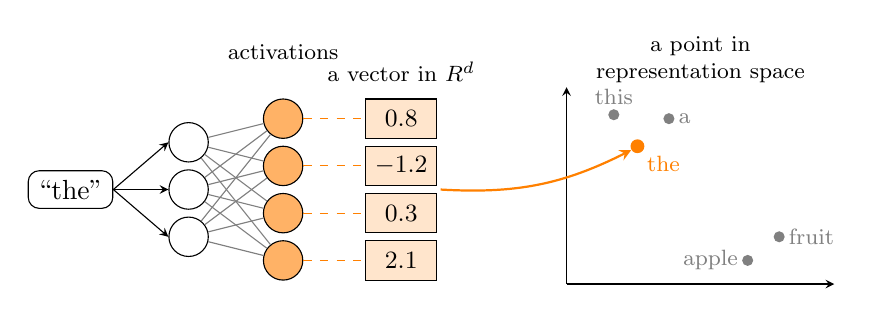
\begin{tikzpicture}[
  >=stealth,
  neuron/.style={circle,draw,minimum size=5mm,inner sep=0pt},
  act/.style={circle,draw,fill=orange!60,minimum size=5mm,inner sep=0pt},
  cell/.style={draw,fill=orange!20,minimum width=9mm,minimum height=5mm,font=\small},
  lab/.style={font=\footnotesize,align=center}
]
% input word
\node[draw,rounded corners] (in) at (0,0) {``the''};

% first layer
\foreach \i/\y in {1/0.6,2/0,3/-0.6}
  \node[neuron] (a\i) at (1.5,\y) {};

% hidden layer (the activations)
\foreach \i/\y in {1/0.9,2/0.3,3/-0.3,4/-0.9}
  \node[act] (h\i) at (2.7,\y) {};

% connections
\foreach \i in {1,2,3}
  \draw[->] (in.east) -- (a\i.west);
\foreach \i in {1,2,3}
  \foreach \j in {1,...,4}
    \draw[gray] (a\i) -- (h\j);

% activation vector
\foreach \j/\v/\y in {1/0.8/0.9,2/-1.2/0.3,3/0.3/-0.3,4/2.1/-0.9}
  \node[cell] (v\j) at (4.2,\y) {$\v$};
\foreach \j in {1,...,4}
  \draw[dashed,orange] (h\j.east) -- (v\j.west);

% representation space
\draw[->] (6.3,-1.2) -- (9.7,-1.2);
\draw[->] (6.3,-1.2) -- (6.3,1.3);

\fill[orange] (7.2,0.55) circle (2.5pt) node[below right,font=\footnotesize] {the};
\fill[gray] (7.6,0.9) circle (2pt) node[right,font=\footnotesize] {a};
\fill[gray] (6.9,0.95) circle (2pt) node[above,font=\footnotesize] {this};
\fill[gray] (9.0,-0.6) circle (2pt) node[right,font=\footnotesize] {fruit};
\fill[gray] (8.6,-0.9) circle (2pt) node[left,font=\footnotesize] {apple};

\draw[->,thick,orange] (4.7,0) to[bend right=15] (7.12,0.5);

% labels
\node[lab] at (2.7,1.75) {activations};
\node[lab] at (4.2,1.50) {a vector in $\mathbb{R}^d$};
\node[lab] at (8.0,1.65) {a point in\\ representation space};
\end{tikzpicture}
\end{frame}

\begin{frame}
\frametitle{Unsupervised learning}
\vskip 0.25cm
In supervised learning we have data points and labels and we try to learn how to map from data to labels.
\vskip 0.5cm
In unsupervised learning we just have data points and we try to decide what structure they have, what is interesting about them, before thinking about labelling at all.
\vskip 0.5cm
In real life the distinction is blurry: a neural network is trained on labelled data, but its early layers often do something more like unsupervised learning, breaking the input down by its intrinsic structure, all the better to be classified by later layers.
\end{frame}

\begin{frame}
\frametitle{Why PCA?}
\vskip 0.25cm
Principal component analysis is often the first thing you do when you look at a new data set.
\vskip 0.5cm
It is also an early demonstration of a big idea: data usually has structure, and this is why AI works as well as it does!
\vskip 0.5cm
Keep in mind that many interesting aspects of neural networks, autoencoders for example, are understandable as non-linear generalizations of PCA.
\end{frame}

\begin{frame}
\frametitle{Some data}
\begin{columns}[c]
\begin{column}{0.5\textwidth}
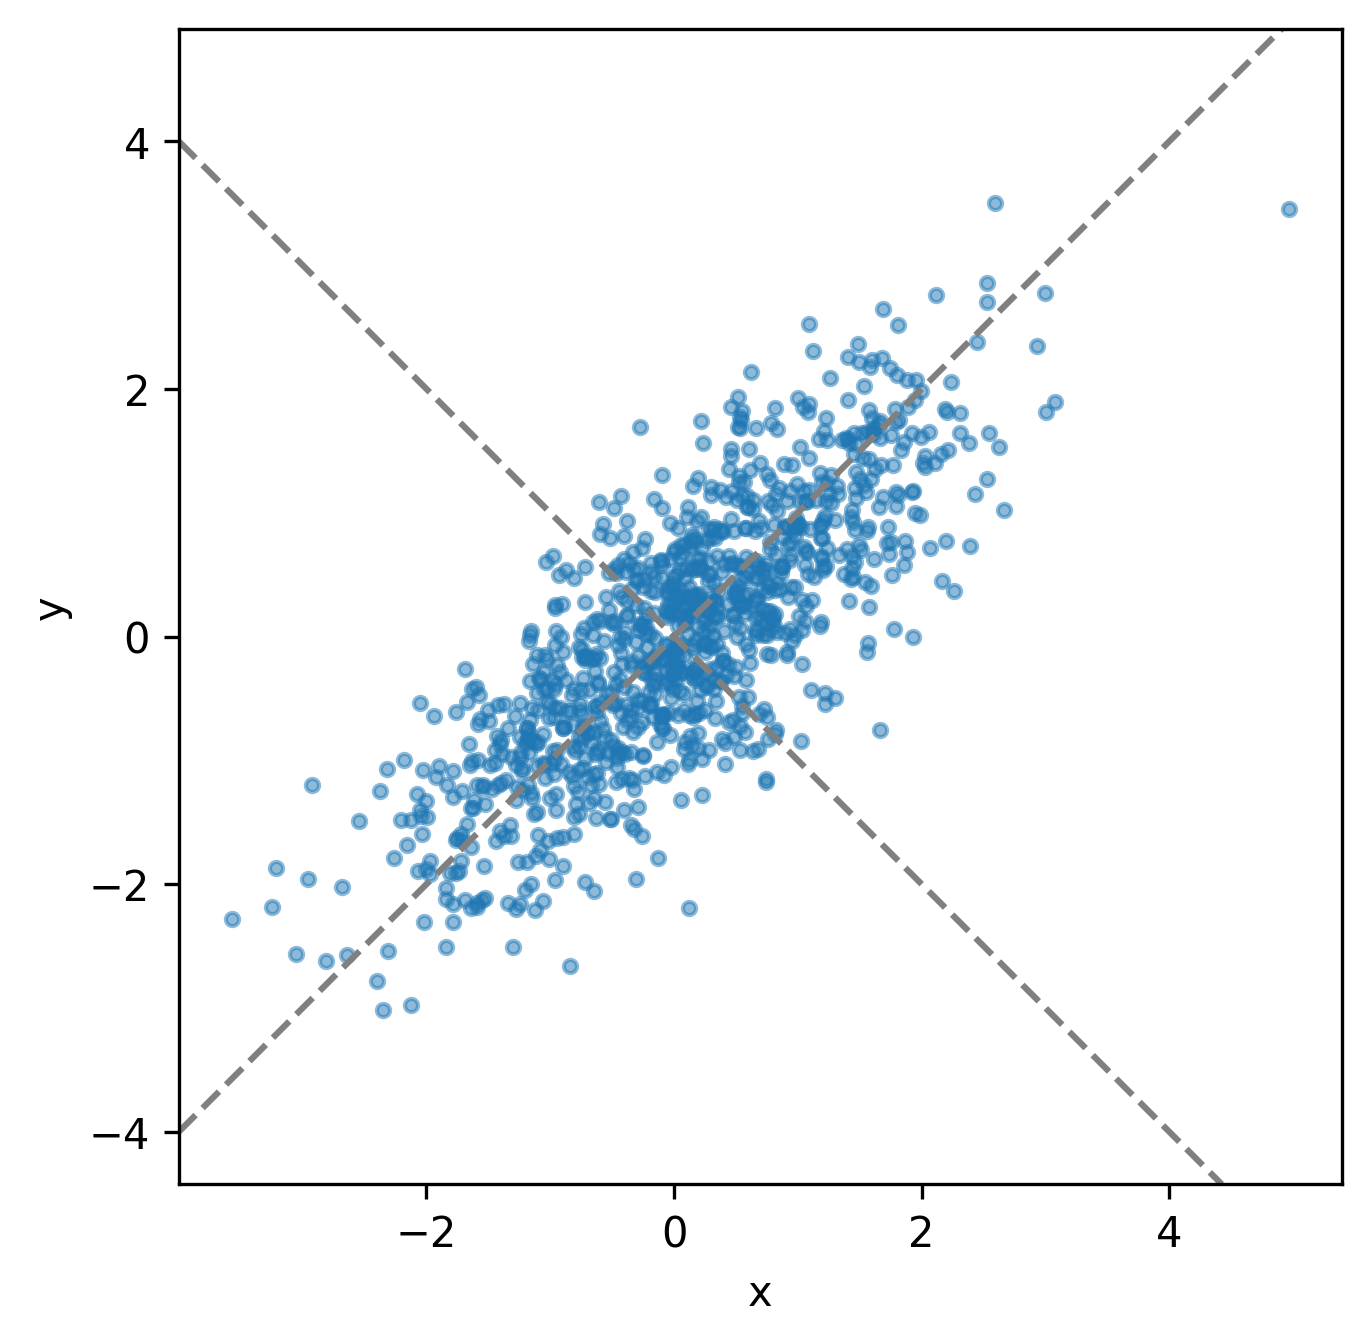
\includegraphics[width=\textwidth]{anisotropic_gaussian.png}
\end{column}
\begin{column}{0.5\textwidth}
Say we have measured lots of people's ears: $x$ is the size of the left ear, $y$ the size of the right ear, with the average removed.
\vskip 0.5cm
The $x=y$ direction measures ``how big is the person'' and the $x=-y$ direction measures ``how symmetric is the person''.
\end{column}
\end{columns}
\end{frame}

\begin{frame}
\frametitle{Finding the structure}
\vskip 0.25cm
The data are spread out along the $x=y$ direction with a bit of ``blurring'' along the $x=-y$ direction.
\vskip 0.5cm
In an experiment $x=y$ might be the phenomenon and $x=-y$ the noise, so you might want to ignore $x=-y$ and project the points onto $x=y$.
\vskip 0.5cm
Here we can see the structure by eye; discovering it automatically, in any number of dimensions, is the business of PCA.
\end{frame}

\begin{frame}
\frametitle{The covariance matrix}
\vskip 0.25cm
The first thing to look at is the covariance matrix
$$
\Sigma=\mathbb{E}\left[(\mathbf{x}-\boldsymbol{\mu})(\mathbf{x}-\boldsymbol{\mu})^{\mathsf T}\right]
$$
which, in practice, we estimate from data:
$$
\hat{\Sigma}_{ij}=\frac{1}{n-1}\sum_{k=1}^{n}\bigl(x_i^{(k)}-\bar{x}_i\bigr)\bigl(x_j^{(k)}-\bar{x}_j\bigr)
$$
``Co-'' means with: $\Sigma_{12}$ measures how much $x_1$ and $x_2$ vary together.
\end{frame}

\begin{frame}
\frametitle{Covariance and independence}
\vskip 0.25cm
If two variables are independent the corresponding entry in the covariance matrix is zero, though the sample covariance might give a small value.
\vskip 0.5cm
The converse isn't true: zero covariance does not imply independence, you need the mutual information for that!
\end{frame}

\begin{frame}
\frametitle{Our example}
\vskip 0.25cm
For the ear data
$$
\hat{\Sigma}=\begin{pmatrix}
1.21 & 0.92\\
0.92 & 1.12
\end{pmatrix}
$$
so 1.21 is the variance in the $x$ direction, 1.12 in the $y$ direction and 0.92 is how much $x$ and $y$ vary together.
\vskip 0.5cm
What we want are the directions where the covariance matrix is diagonal: where the variables don't vary together.
\end{frame}

\begin{frame}
\frametitle{Diagonalizing}
\vskip 0.25cm
A covariance matrix is symmetric, so it can be diagonalized
$$
\Sigma=PDP^{\mathsf T}
$$
where $D$ is diagonal with the eigenvalues and the columns of $P$ are the unit eigenvectors.
\vskip 0.5cm
For our example, $\lambda_1\approx 2.08$ with $\mathbf{e}_1\approx(1,1)^{\mathsf T}$ and $\lambda_2\approx 0.24$ with $\mathbf{e}_2\approx(1,-1)^{\mathsf T}$:
$$
\hat{\Sigma}\approx\frac{1}{2}
\begin{pmatrix}1 & 1\\1 & -1\end{pmatrix}
\begin{pmatrix}2.08 & 0\\0 & 0.24\end{pmatrix}
\begin{pmatrix}1 & 1\\1 & -1\end{pmatrix}^{\mathsf T}
$$
\end{frame}

\begin{frame}
\frametitle{New axes}
\vskip 0.25cm
With the average removed, $\Sigma_\mathbf{x}=\mathbb{E}[\mathbf{x}\mathbf{x}^{\mathsf T}]$. Now change variables, $\mathbf{x}=P\mathbf{y}$:
$$
\Sigma_\mathbf{x}
=\mathbb{E}\left[P\mathbf{y}\mathbf{y}^{\mathsf T}P^{\mathsf T}\right]
=P\,\mathbb{E}\left[\mathbf{y}\mathbf{y}^{\mathsf T}\right]P^{\mathsf T}
=P\Sigma_\mathbf{y}P^{\mathsf T}
$$
\vskip 0.25cm
So diagonalizing the covariance matrix finds new axes in which the covariance is diagonal. These new axes are the \emph{principal components}.
\end{frame}

\begin{frame}
\frametitle{Loadings and scores}
\vskip 0.25cm
The columns of
$$
P=[\hat{\mathbf{e}}_1,\hat{\mathbf{e}}_2,\ldots,\hat{\mathbf{e}}_n]
$$
are the \emph{loading vectors}: each tells you which original variables contribute to that component, and how strongly.
\vskip 0.5cm
The coordinates of a data point in the new axes
$$
\mathbf{y}=P^{\mathsf T}\mathbf{x}
$$
are the \emph{principal component scores}: the same data, rotated.
\end{frame}

\begin{frame}
\frametitle{Interpretation}
\vskip 0.25cm
PCA doesn't give you an interpretation, it just finds the components.
\vskip 0.5cm
We know $x_1$ and $x_2$ are the sizes of the left and right ears; it is up to us to decide that $y_1$ is ``how big the person is'' and $y_2$ is ``how symmetric the person is''.
\vskip 0.5cm
Since most of the variance comes from $y_1$, we might decide to ignore $y_2$.
\end{frame}

\begin{frame}
\frametitle{Dimensionality reduction}
\vskip 0.25cm
We can rotate back: $\mathbf{x}=P\mathbf{y}$.
\vskip 0.5cm
If we keep only the first $m$ components, the ones with the largest eigenvalues, $P_m=[\hat{\mathbf{e}}_1,\ldots,\hat{\mathbf{e}}_m]$, then
$$
\mathbf{y}_m=P_m^{\mathsf T}\mathbf{x},
\qquad
\mathbf{x}\approx P_m\mathbf{y}_m
$$
so we represent each data point with only $m$ numbers while losing as little variance as possible.
\end{frame}

\begin{frame}
\frametitle{A health warning}
\vskip 0.25cm
This is a particularly clean example: the ``blur'' is completely independent of the ``signal''.
\vskip 0.5cm
Often PCA is a best guess at the directions along which things happen independently, but these directions may not exist, or may not be perpendicular.
\vskip 0.5cm
PCA is then only a first step before more non-linear methods, such as ICA or a neural network, an autoencoder for example.
\end{frame}

\begin{frame}
\frametitle{Covariance or correlation?}
\vskip 0.25cm
Use the covariance if the units are the same for all the dimensions and the variances are comparable.
\vskip 0.5cm
Otherwise use the correlation matrix, the covariance rescaled by the standard deviations:
$$
R_{ij}=\frac{\Sigma_{ij}}{\sqrt{\Sigma_{ii}\Sigma_{jj}}}
$$
\end{frame}

\begin{frame}
\frametitle{Independent component analysis}
\vskip 0.25cm
PCA is everywhere and easy to describe. ICA is often more useful but harder to explain: there isn't really a single well-defined algorithm for finding the independent components.
\vskip 0.5cm
The real message is about representation: changing how data is encoded as a vector can disentangle its structure.
\end{frame}

\begin{frame}
\frametitle{PCA versus ICA}
\begin{columns}[t]
\begin{column}{0.5\textwidth}
\centering
\textbf{PCA}\\[2pt]
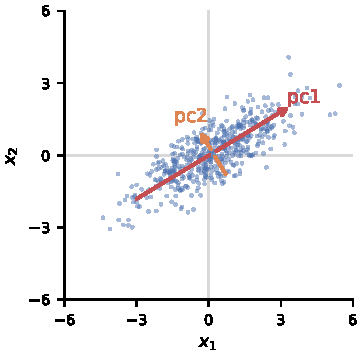
\includegraphics[width=\linewidth]{pca.pdf}
\end{column}
\begin{column}{0.5\textwidth}
\centering
\textbf{ICA}\\[2pt]
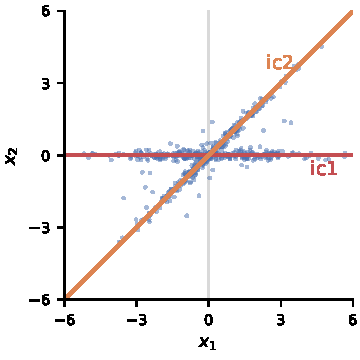
\includegraphics[width=\linewidth]{ica.pdf}
\end{column}
\end{columns}
\vskip 0.25cm
PCA finds orthogonal axes ordered by variance; ICA finds the directions, not necessarily orthogonal, along which the data are independent.
\end{frame}

\begin{frame}
\frametitle{Ginger and garlic}
\vskip 0.25cm
Measure how much garlic ($x$) and ginger ($y$) are in lots of recipes.
\vskip 0.5cm
Italian recipes: the garlic varies, but there is hardly any ginger.
\vskip 0.25cm
Indian recipes: garlic and ginger in roughly equal amounts, lots of both or a little of both.
\vskip 0.5cm
So there is a discrete choice, the cuisine, and then a continuous process that depends on it. The two arms are the \emph{independent components}.
\end{frame}

\begin{frame}
\frametitle{The cocktail party problem}
\vskip 0.25cm
Two people talking, each ear hears a different weighted mix of the two voices.
\vskip 0.5cm
Two independent sources, two observed mixtures: the job of ICA is to separate the mixtures back into the two voices.
\vskip 0.5cm
This isn't really how we do it, but there are versions of the problem where fastICA is exactly what is used.
\end{frame}

\begin{frame}
\frametitle{Mixing}
\vskip 0.25cm
Independent, non-Gaussian sources $X_1$ and $X_2$ are mixed:
$$
\begin{pmatrix}Y_1\\Y_2\end{pmatrix}=M\begin{pmatrix}X_1\\X_2\end{pmatrix}
$$
We want an unmixing matrix $W$:
$$
\begin{pmatrix}Z_1\\Z_2\end{pmatrix}=W\begin{pmatrix}Y_1\\Y_2\end{pmatrix}=WM\begin{pmatrix}X_1\\X_2\end{pmatrix}
$$
If $W=M^{-1}$ then $Z_i=X_i$ and we have recovered the sources.
\end{frame}

\begin{frame}
\frametitle{The trick behind fastICA}
\vskip 0.25cm
The central limit theorem gives a vague lesson: adding random things up gives something more Gaussian than the things themselves.
\vskip 0.5cm
So the mixtures $Y_i$ are more Gaussian than the sources $X_i$.
\vskip 0.5cm
fastICA varies $W$ to make the $Z_i$ as \emph{un}-Gaussian as possible: the less mixed, the less Gaussian.
\end{frame}

\begin{frame}
\frametitle{Words as vectors}
\vskip 0.25cm
word2vec maps words to vectors: a one-hot vector for each word is mapped to a 300-dimensional latent space and then to predictions of which words appear nearby.
\vskip 0.5cm
The latent vectors $\mathbf{v}[\text{word}]$ seem to capture aspects of meaning:
$$
\mathbf{v}(\text{Mozart})+[\mathbf{v}(\text{scientist})-\mathbf{v}(\text{Einstein})]\approx\mathbf{v}(\text{violinist})
$$
These examples were cherry-picked, but it was cool at the time!
\end{frame}

\begin{frame}
\frametitle{ICA on GloVe}
\vskip 0.25cm
GloVe is a standard, downloadable set of 100-dimensional word vectors.
\vskip 0.5cm
Take the twenty thousand or so most common words, leaving out the hundred commonest, and treat each word's vector as a data point, just like the recipes.
\vskip 0.5cm
Run fastICA asking for 100 components; to see what a component is ``about'', list the words with the largest values along it.
\end{frame}

\begin{frame}
\frametitle{Food and music}
\begin{columns}[c]
\begin{column}{0.5\textwidth}
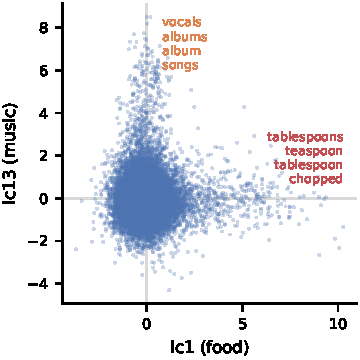
\includegraphics[width=\textwidth]{ica_words.pdf}
\end{column}
\begin{column}{0.5\textwidth}
Plotted against two independent components, the words make the same two-armed picture as the recipes.
\vskip 0.5cm
Food words along one axis, music words along the other and almost nothing in between: most words are mostly about one thing.
\end{column}
\end{columns}
\end{frame}

\begin{frame}
\frametitle{Some components}
\vskip 0.25cm
\begin{itemize}
\item \textbf{cooking:} teaspoon, tablespoons, sauce, garlic, chopped
\item \textbf{music:} albums, vocals, songs, band, guitar, jazz
\item \textbf{stock markets:} Topix, DAX, KOSPI, FTSE, Nikkei
\item \textbf{computing:} desktop, Macintosh, Android, USB, software
\item \textbf{injuries:} spinal, ligament, knee, ankle, tendon
\end{itemize}
\vskip 0.5cm
Some components are about grammar or style instead: intensifiers like incredibly, utterly, extremely; verbs ending in ``-ing''. A few are junk.
\end{frame}

\begin{frame}
\frametitle{PCA is messier}
\vskip 0.25cm
Do the same with PCA and the lists are a jumble: a few components are coherent, but one, for example, has Ingushetia, the Sensex stock index, the PKK and landslides.
\vskip 0.5cm
ICA knows nothing about language, it only looks for directions along which the data is as un-Gaussian as possible, yet it pulls out much of the structure of meaning.
\end{frame}

\end{document}